\section{Conceptual Design and Justification}

The conceptual design of the Micromouse was guided by a central systems-engineering question: which overall architecture offers the highest probability of reliable autonomous maze navigation under realistic project constraints. In this context, the challenge was not simply to select individual components, but to define a coherent concept in which sensing, actuation, computation, and software structure support one another. The resulting design therefore prioritised robustness, controllability, and ease of integration over maximum competition speed.

At system level, three criteria were considered particularly important. First, the robot had to be controllable, meaning that commanded motions such as straight driving and turning should be repeatable despite disturbances and asymmetries. Second, it had to be observable, meaning that both the environment and the robot motion should be measurable with sufficient reliability for navigation. Third, it had to be implementable, meaning that the hardware and software complexity should remain compatible with the available time, budget, and manufacturing resources. The final concept was selected as a compromise that satisfies these three requirements simultaneously.

\subsection{Design Requirements and Constraints}

From a functional point of view, the robot had to fulfil several basic requirements:
\begin{itemize}
    \item autonomous movement in a cell-based maze,
    \item reliable wall detection at the left, front, and right side,
    \item sufficiently accurate straight driving and turning,
    \item storage of the explored maze structure,
    \item execution of a goal-directed run based on the generated map,
    \item practical support for debugging and commissioning.
\end{itemize}

In addition to these functional requirements, the project was subject to clear practical constraints. It had to be realised as an academic prototype within limited development time and with a moderate component budget. For this reason, the design objective was not to reproduce a fully competition-optimised Micromouse system, but to realise a complete and technically well-justified autonomous platform. This also affected the problem scope. While the classical Micromouse problem is defined on a {16 x 16} maze, the implemented system uses a reduced {6 x 6} maze representation together with a predefined goal configuration. This reduction in problem size was justified because it allowed development effort to be concentrated on the essential system-integration tasks of sensing, control, localisation, and map-based navigation.

Figure~\ref{fig:test_maze} shows the physical reduced maze used for the project. Including this reduced maze in the report is useful because it makes the practical task definition more concrete and helps the reader judge the achieved system behaviour against the intended project scope.

\begin{figure}[t]
    \centering
    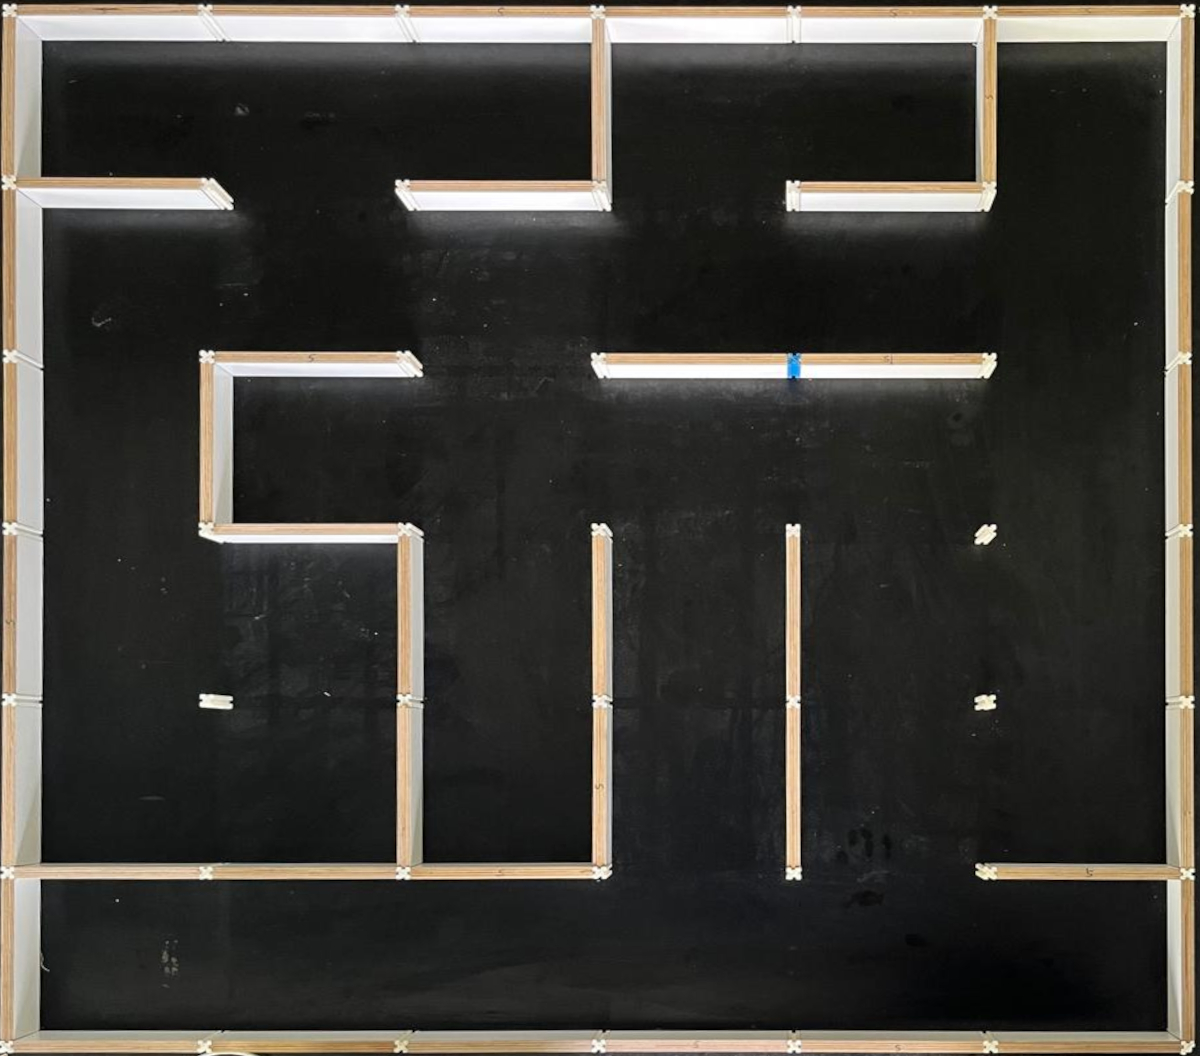
\includegraphics[width=0.8\columnwidth]{images/maze.jpeg}
    \caption{Reduced maze used for the implemented Micromouse project.}
    \label{fig:test_maze}
\end{figure}

\subsection{Locomotion Concept}

The selected locomotion concept is a differential-drive robot with two independently actuated drive wheels. This arrangement is particularly appropriate for maze navigation because it combines mechanical simplicity with sufficient manoeuvrability. In contrast to steering-based concepts, no additional steering mechanism is required. In contrast to omnidirectional solutions, the drivetrain remains simple, compact, and easy to model. The robot can therefore execute the fundamental maze manoeuvres directly: straight motion, left and right turns, and turning on the spot.

From a control perspective, the differential-drive concept is advantageous because it reduces the motion problem to the coordinated control of two wheel velocities. However, this benefit only holds if wheel motion is measured. For that reason, wheel encoders were included as an essential part of the concept rather than as an optional refinement. They provide the feedback needed for closed-loop speed regulation, estimation of travelled distance, and monitoring of turn progress. Without this feedback, the robot would depend excessively on open-loop actuation and would accumulate unacceptable motion errors during repeated cell transitions.

\subsection{Sensing Concept}

The sensing concept combines three infrared distance sensors with incremental wheel encoders. The infrared sensors provide environmental information, while the encoders provide motion information. This distinction is important at conceptual level, because successful maze navigation depends both on knowing where walls are and on estimating how the robot itself has moved.

The infrared sensors were arranged to observe the left, front, and right directions. This layout was selected because it captures the minimum external information required for the intended navigation task. The side sensors provide a reference for wall following and lateral correction during straight driving, while the front sensor supports wall detection ahead of the robot and contributes to the interpretation of cell transitions. A larger sensor set could in principle improve redundancy or geometric reconstruction, but it would also increase electrical complexity, software effort, and calibration requirements. For the intended project scope, three sensors represented an effective balance between information content and implementation effort.

The encoders complement the infrared sensors by providing a measure of wheel rotation and therefore of speed and travelled distance. Conceptually, this creates a combined sensing architecture in which external measurements are used to interpret maze structure and internal measurements are used to estimate motion. Such a combination is more robust than relying on only one of the two sensing modalities. Infrared sensing alone would not provide reliable motion estimation, whereas odometry alone would not detect walls or corridor geometry.

\subsection{Embedded Hardware Concept}

The hardware concept is centred around a dedicated microcontroller-based PCB that integrates the major functional subsystems of the robot. This choice was justified by the need for a compact, electrically consistent, and mechanically manageable platform. A single-board design reduces wiring effort, improves reproducibility, and lowers the risk of intermittent faults that commonly arise in loosely wired prototypes. It also supports a cleaner separation between power electronics, sensing, communication, and logic-level processing.

The implemented embedded platform is based on a dsPIC-centered controller board together with a dual H-bridge motor driver, analogue infrared sensors, voltage regulation stages, user-interface elements, and a wireless communication module. At conceptual level, such a microcontroller-based platform is well suited to the application because it combines the peripheral capabilities that are particularly relevant for this task: pulse-width modulation for motor actuation, analogue-to-digital conversion for sensor acquisition, quadrature encoder support for motion feedback, timers and interrupts for real-time scheduling, and serial communication for debugging. By concentrating these functions in one controller, the design remains comparatively compact and avoids unnecessary interface overhead.

The power architecture follows the same logic of functional integration. Since the drive system and the logic-level electronics have different electrical requirements, voltage regulation is necessary to provide stable operating conditions for sensors, communication hardware, and control electronics. In addition, wireless UART communication was included as part of the concept because a mobile robot benefits strongly from untethered debugging during experiments in the maze. Although this feature is not strictly required for autonomous motion, it significantly improves observability during development and therefore supports the practical implementation process.

\subsection{Software and Navigation Concept}

The software concept follows a layered architecture in which hardware access, motion control, and navigation logic are separated into distinct levels of abstraction. This structure was chosen because the project combines tasks of very different character. At lower level, the software must handle peripheral configuration, sensor acquisition, and actuator output. On top of this, the control functions regulate wheel motion and provide reusable movement primitives, while the navigation layer represents the maze, decides where to move next, and manages the transition between exploration and goal-directed motion. A layered design reduces coupling between these concerns and thereby improves maintainability and testability.

At navigation level, a map-based approach was selected instead of a purely reactive one. This decision is conceptually important. A reactive robot can avoid immediate obstacles, but it does not necessarily solve a maze efficiently or even correctly when revisiting already explored regions. By contrast, a map-based approach allows the robot to store cell connectivity, distinguish between local sensor observations and global maze orientation, and compute paths through already known territory. This is much more suitable for a Micromouse-type task, where successful behaviour depends not only on instantaneous wall detection but also on memory and route selection.

The chosen strategy therefore consists of two logically separate phases. In the first phase, the robot explores the accessible maze and constructs an internal representation of the discovered cell connections. In the second phase, this stored representation is used to drive toward a predefined goal. This division is justified because it separates the difficult task of acquiring environmental knowledge from the later task of exploiting that knowledge. It also reflects a clear experimental structure: the first run evaluates sensing, localisation, and map consistency, whereas the second run evaluates the usefulness of the generated map for purposeful navigation.

\subsection{Justification of the Overall Approach}

Taken as a whole, the selected concept is justified not because each individual element is maximally sophisticated, but because the elements fit together in a technically coherent way. The differential-drive arrangement provides a simple and controllable mechanical basis. The encoder and infrared sensor combination provides the minimum feedback necessary for closed-loop motion and wall-based interpretation of the maze. The microcontroller-based PCB supplies the required embedded functionality in a compact implementation. The layered software structure and map-based navigation strategy provide an appropriate computational framework for autonomous maze traversal.

This makes the overall design well suited to the aims of the project. Rather than pursuing a narrowly optimised high-speed competition robot, the concept emphasises the successful integration of electronics, embedded software, control, and navigation into a complete autonomous system. Such a design is particularly appropriate in an academic context, because it exposes the main engineering trade-offs clearly while remaining feasible to implement, test, and evaluate in a rigorous manner. The following chapters build on this conceptual basis by describing the detailed hardware and software realisation and the implemented controller design.
